\documentclass[border=10pt,tikz,multi]{standalone}
\usetikzlibrary{angles,shadows.blur,positioning,backgrounds}

\begin{document}
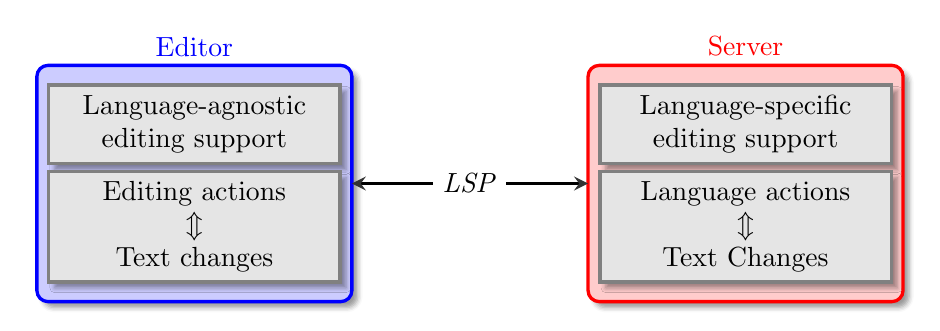
\begin{tikzpicture}
% \draw[blue, very thick, rounded corners, fill=blue!20, anchor=north, blur shadow={shadow blur steps=5}]
\draw[blue, very thick, rounded corners, fill=blue!20, anchor=north, blur shadow]
        (0,0) rectangle (4,3)
        node[anchor=north, align=center] at (2,3.5) {Editor};
\draw[gray, very thick, fill=gray!20, blur shadow]
        (0.15, 1.75) rectangle (3.85,2.75)
        node[black, text width=4cm, pos=.5, align=center] {Language-agnostic \linebreak editing support};
\draw[gray, very thick, fill=gray!20, blur shadow]
        (0.15, 0.25) rectangle (3.85,1.65)
        node[black, text width=4cm, pos=.5, align=center] {Editing actions \linebreak $\Updownarrow$ \linebreak  Text changes};

\draw[red, very thick, rounded corners, fill=red!20, anchor=north, blur shadow]
        (7,0) rectangle (11,3)
        node[anchor=north, align=center] at (9,3.5) {Server};
\draw[gray, very thick, fill=gray!20, blur shadow]
        (7.15, 1.75) rectangle (10.85,2.75)
        node[black, text width=4cm, pos=.5, align=center] {Language-specific \linebreak editing support};
\draw[gray, very thick, fill=gray!20, blur shadow]
        (7.15, 0.25) rectangle (10.85,1.65)
        node[black, text width=4cm, pos=.5, align=center] {Language actions \linebreak $\Updownarrow$ \linebreak Text Changes};

\draw[<->, very thick, >=stealth] (4,1.5) -- (7,1.5)
        node[midway,fill=white] {\emph{LSP}};
\end{tikzpicture}
\end{document}
